\chapter{Theoretical Background}
\section{Basics in Modeling Light in Computer Graphics}

\subsection{Radiometry}
One purpose of Computer Graphics is to simulate the interaction of light on a surface and how a real-world observer, such as a human eye, will perceive this. These visual sensations of an eye are modeled relying on a virtual camera which captures the emitted light from the surface. The physical basis to measure such reflected light depicts radiometry which is about measuring the electromagnetic radiation transfered from a soruce to a receiver. 

Fundamentally, light is a form of energy propagation, consisting of a large collection of photons, whereat each photon can be considered as a quantum of light that has a position, direction of propagation and a wavelength $\lambda$. A photon travels at a certain speed $v = \frac{c}{n}$, that depends only the speed of light $c$ and the refractive index $n$ through which it progrates. Its frequency is defined by $f = \frac{v}{\lambda}$ and its carried amount of energy $q$, mearsured in the SI unit Joule, is given by $q = hf= \frac{hv}{\lambda n}$ where $h$ is the Plank's constant. The total energy of a large collection of photons is hence $Q = \sum_i q_i$.

\subsection{Spectral Energy}

It is important to understand that the human eye is not equally sensitive to all wavelength of the spectrum of light and therefore responds differently to specific wavelengths. Remember that our goal is to model the human visual perception. This is why we consider the energy distribution of a light spectrum rather than considering the total energry of a photon collection since then we could weight the distribution according the human visual system. So the question we want to answer is: How is the energy distributed across wavelengths of light?

The idea is to make an energy histrogram from a given photon collection. For this we have to order all photons by their associated wavelength, discretize wavelength spectrum, count all photons which then will fall in same wavelength-interval, and then, finally, normalize each interval by the total energy $Q$. This will give us a histogram which tells us the spectral energy $Q_{\lambda}$ for a given discrete $\lambda$ interval and thus models the so called spectral energy distribution $\footnote{Intensive quantities can be thought of as density functions that tell the density of an extensive quantity at an infinitesimal point.}$.

\subsection{Spectral Power}
Rendering an image in Computer Graphics corresponds to capturing the color sensation of an illuminated, target scene at a certain point in time. As previousely seen, each color is associated by a wavelength and is directly related to a certain amount of enegry. In order to determine the color of a to-be-rendered pixel of an image, we have to get a sense of how much light (in terms of energy) passes through the area which the pixel corresponds to. One possibility is to consider the flow of energy $\Phi = \frac{\Delta Q}{\Delta t}$ transferred through this area over a small period of time. This allows us to measure the energy flow through a pixel during a certain amount of time. 

In general, power is the estimated rate of energy production for light sources and corresponds to the flux. It is measured in the unit Watts, denoted by Q. Since power is a rate over time, it is well defined even when energy production is varying over time. As with Spectral Energy for rendering, we are really interested in the spectral power $\Phi_\lambda = \frac{\Phi}{\lambda}$, measured in Watts per nanometer.

\subsection{Spectral Irradiance}
Before we can tell how much light is reflected from a given point on a surface towards the viewing direction of an observer, we first have to know how much light arrives at this point. Since in general a point has no length, area or even volume associated, let us instead consider an infinitimal area $\Delta A$ around a such a point. Then, we can ask ourself how much light falls in such a small area. When further observing this process over a short period in time, this quantity is the spectral irradiance $E$ as illustrated in figure $\ref{fig:irradiance}$. Summarized, this quantity tells us how much spectral power is incident on a surface per unit area and mathematically is equal:

\begin{equation}
 E = \frac{\Phi_{\lambda}}{\Delta A}
\end{equation} 

\begin{figure}[H]
  \centering
  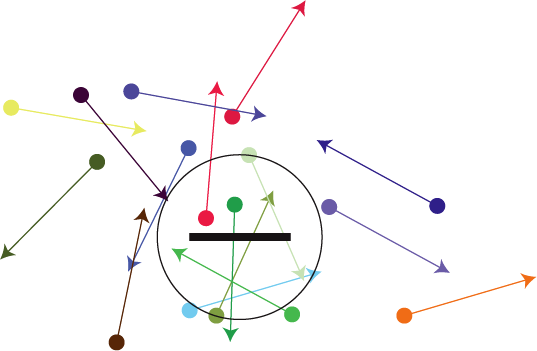
\includegraphics[scale=0.5]{background/irradiance.png}
  \caption{Irradiance is the summed up radiance over all directions}
  \label{fig:irradiance}
\end{figure}

\subsection{Spectral Radiance}
\subsection{BRDF}
how much light is reflected back from P in a given direction (generally the viewing direction), we first need to know how much light arrives at P from all directions in the hemisphere above the point. 
\subsection{Colorspace}
\subsection{Spectral Rendering}

\section{Wave Theory for Light and Diffraction}
\section{Stam's BRDF formulation}